\documentclass[tikz,border=10pt]{standalone}
\usepackage{tikz}
\usepackage{caption}


\usetikzlibrary{calc}
\usetikzlibrary{positioning}
\usetikzlibrary{shapes.geometric, arrows}
\usetikzlibrary{quantikz}


\tikzstyle{res} = [rectangle, rounded corners,
minimum width=3cm,
minimum height=3cm,
text centered,
draw=black,
fill=blue!30]

\tikzstyle{var} = [rectangle,
minimum width=0cm,
minimum height=0cm,
text centered,
text width=0.5cm,
draw=white,
fill=white!30]

\tikzstyle{arrow} = [thick,->,>=stealth]

\RequirePackage{xcolor}

% Main colour
\definecolor{sintefblue}{HTML}{003C65}

% Contrast colours
\definecolor{sintefcyan}{HTML}{22A7E5}
\definecolor{sintefmagenta}{HTML}{EC008C}
\definecolor{sintefgreen}{HTML}{A4C21F}
\definecolor{sintefyellow}{HTML}{F7E918}

\definecolor{sintefred}{HTML}{BE3C37}

% Additional colours
\definecolor{sintefgrey}{HTML}{A19589}
\colorlet{sintefgray}{sintefgrey}
\definecolor{sinteflightgrey}{HTML}{D8D0C7}
\colorlet{sinteflightgray}{sinteflightgrey}

\def\oosqrt{0.7071067811865475}

\newcommand{\drawqubit}[4][green]{
    \draw[#1,thick] (#2,#3) circle (#4);
    \draw[#1,thick] (-#4+#2,#3) arc (180:360:#4 and 0.5*#4);
    \draw[#1] (-#4+#2,#3) arc (180:0:#4 and 0.5*#4);
    % \draw (-.5*#3+#1,#2+.5*#3) node[anchor=north west] {0};
    % \draw (-.5*#3+#1,#2-.5*#3) node[anchor=north west] {1};
    \draw[#1,very thick,-stealth] (#2,#3) -- (#2+\oosqrt*#4,#3+\oosqrt*#4);
}

\begin{document}
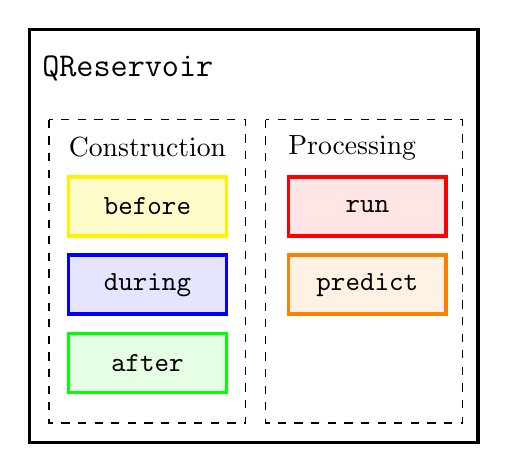
\begin{tikzpicture}[
    resnode/.style={rectangle, very thick, minimum width=2cm, minimum height=0.75cm
    }
]
    \node[resnode, draw=yellow, fill=yellow!20, text=black] (before) {\texttt{before}};
    \node[resnode, draw=blue, fill=blue!10, text=black] (during) [below=0.2cm of before] {\texttt{during}};
    \node[resnode, draw=green, fill=green!10, text=black] (after) [below=0.2cm of during] {\texttt{after}};

    \node[resnode, draw=red, fill=red!10, text=black] (run) [right=.75cm of before] {\texttt{run}};
    \node[resnode, draw=orange, fill=orange!10, text=black] (predict) [right=.75cm of during] {\texttt{predict}};

    \draw[very thick] (-1.5, 2.25) rectangle (4.2, -3.);
    \draw[dashed] (-1.25,  1.1) rectangle (1.25, -2.75);
    \draw[dashed] (1.5,  1.1) rectangle (4, -2.75);

    \node at (-.25, 1.75) {\large \texttt{QReservoir}};
    \node at (-0, 0.75) {Construction};
    \node at (+2.6, 0.75) {Processing};
\end{tikzpicture}
            % \captionof{figure}{A quantum reservoir system consists of a learning task, an en- and de-coder (red) and the dynamic system itself (green). In standard RC the machine learning part is linear regression.
            % }
\end{document}

